\section*{Caracterización de componentes pasivos}

\subsection*{Inductancia}
A continuación, se realizará un estudio acerca del comportamiento de una bobina, observando como varían sus magnitudes según la frecuencia y analizando sus circuitos equivalentes.\par En un sistema simplificado, la bobina sólo tiene un componente inductivo, sin embargo, dicho planteo dista en gran medida de la realidad donde, debido a su fabricación, las inductancias tendrán tanto componentes resistivos como capacitivos. \par Las características previamente mencionadas nos llevarán a plantear distintos circuitos equivalentes. Se analizará cual de ellos refleja en mejor medida la práctica experimental realizada.

Para comenzar, se realiza el estudio de las magnitudes propias del inductor en función de la frecuencia. \par Las frecuencias utilizadas fueron detectadas ya que eran las que permitían ver con claridad como variaba la fase. Las mediciones se tomaron en el modo serie del analizador de impedancias, las mismas se pueden apreciar en la tabla (\ref{table:Rta_en_frecuencia_inductor}).

Se plantea el siguiente circuito equivalente:

%circuito equivalente Inductancia
\begin{figure}[H]
\centering
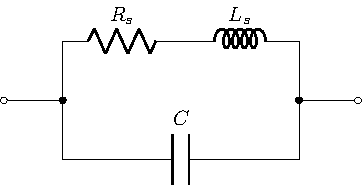
\includegraphics[width=6cm,height=4cm]{Ejercicio_1(Germo)/Circuitos/circuito_equivalente_inductancia.pdf}
\label{fig:circuito_equivalente_inductancia}
\end{figure}
%~circuito equivalente Inductancia

Al ser las bobinas un conjunto de espiras enrolladas una gran cantidad de vueltas, el componente resistivo de la inductancia se debe a la resistencia eléctrica del material utilizado en su fabricación. También, se podría considerar la resistencia propia de los terminales.
Por otro lado, debido a que consctructivamente cada una de las vueltas de la bobina están aisladas eléctricamente entre si debido al barniz que recubre el material y a la pequeña diferencia de tensión, se puede apreciar el comportamiento de un capacitor entre vuelta y vuelta del cable.


%% Tabla inductor
 \begin{center}
     \begin{table}[H]
     \centering
     \renewcommand{\arraystretch}{1.1}
     \scalebox{0.8}{
         \begin{tabular}{ c c c c c c }
            \hline 
             $\bm{f_S[Hz]}$ &  $\bm{L_S[mH]}$ & $\bm{Q}$& $\bm{R_S[\Omega]}$ & $\bm{|Z|[\Omega]}$ & $\bm{\theta}[^\circ]$ \\
             \hline
                10		& 0.490        & 0.0    & 0.91 		& 0.96  & 18.7   \\
				100 	& 0.480       & 3.0   	 & 0.10  	& 0.32  & 72.0     \\
				1K    & 0.480         & 16.6	& 0.18 		& 3.02  & 86.0     \\
				5K    & 0.485        & 25.8 	& 0.59		 & 15.23 & 87.8   \\
				10K   & 0.482        & 26.0     & 1.16 		& 30.32 & 87.8   \\
				20K   & 0.478       & 23.8 		& 2.52 		& 60.11 & 87.6   \\
				30K   & 0.474       & 22.1 		& 4.04 		& 89.35 & 87.4  \\
				50K   & 0.467        & 19.5		 & 7.50 		 & 146.70 & 87.1  \\
				75K   & 0.462       & 16.7 		& 13.00   	& 217.80 & 86.6  \\
				100K  & 0.459       & 14.4 		& 20.00  	 & 289.20 & 86.0   \\
				200K  & 0.466       & 8.6  		& 67.70 	& 589.50 & 83.4    \\
				400K  & 0.529        & 4.1 		 & 322 		 & 1368  & 76.4   \\
				450K  & 0.556        & 3.5 		 & 450  	& 1635  & 74.1   \\
				500K  & 0.589        & 2.9 		 & 632 		 & 1954  & 71.2  \\
				550K  & 0.627        & 2.4  	& 893  		& 2344  & 67.6    \\
				600K  & 0.669        & 2.0    & 1281 		& 2829  & 63.1   \\
				650K  & 0.708        & 1.5 		 & 1868 	& 3442  & 57.1    \\
				700K  & 0.724       & 1.2  		& 2763 		& 4217  & 49.1    \\
				725K  & 0.711        & 1.0  	  & 3356	 & 4664  & 44.0    \\
				750K  & 0.671       & 0.8 		 & 4060 	& 5147  & 38.0    \\
				775K  & 0.595       & 0.6 		 & 4831 	& 5633  & 31.0       \\
				800K  & 0.472       & 0.4 		 & 5608 	& 6089  & 22.9       \\
				825K  & 0.301       & 0.2  		& 6264 		& 6456  & 14.0       \\
				850K  & 0.094        & 0.1  	& 6653		& 6672  & 4.4        \\
				855K  & 0.053       & 0.0  		  & 6692	 & 6698  & 2.5        \\
				862K5 & -0.100         & 0.0    & 6715 		& 6715  & -0.5       \\
				870K  & -0.719       & 0.1 		 & 6706 	& 6718  & -3.4        \\
				875K  & -0.111      & 0.1  		& 6677 		& 6705  & -5.3       \\
				900K  & -0.290      & 0.3  		& 6356 		& 6563  & -14.4      \\
				925K  & -0.421      & 0.4 		 & 5787		 & 6282  & -22.9      \\
				950K  & -0.500         & 0.6  	& 5114 		& 5921  & -30.3       \\
				1M    & -0.549      & 0.9  		& 3820		 & 5146  & -42.1      \\
				1M1  & -0.470      & 1.5  		& 2132		 & 3884  & -56.7      \\
				1M2  & -0.368      & 2.1  		& 1306 		& 3068  & -64.8      \\
				1M3   & -0.291      & 2.7  		& 874  		& 2531  & -69.8      \\
				1M4  & -0.235      & 3.3 		 & 626  	& 2159  & -73.2     \\
				2M    & -0.093      & 6.7 		 & 175 		 & 1179  & -81.5       \\
				4M    & -19.79$\mu$  & 16.8 		& 29.6		 & 498.4 & -86.6     \\
				10M   & -2.893$\mu$ & 27.3 		& 6.7  		& 181.9 & -87.9     \\
            \hline 
        \end{tabular}
        }
        \caption{Magnitudes del inductor en función de la frecuencia}
        \label{table:Rta_en_frecuencia_inductor}
    \end{table}
\end{center}
%%~Tabla inductor

\subsection{Capacitor}
Se procederá a realizar el mismo análisis planteado anteriormente para una inductancia pero, para este caso con un capacitor, analizando como varían sus magnitudes según la frecuencia a la que trabaja y el estudio de sus circuitos equivalentes.

Para comenzar, se realiza el estudio de las magnitudes propias del capacitor en función de la frecuencia. \par Las frecuencias utilizadas fueron detectadas ya que eran las que permitían ver con claridad como variaba la fase. Las mediciones se tomaron en el modo paralelo del analizador de impedancias por lo que se medirán conductancias. Las mismas se pueden apreciar en la tabla (\ref{table:Rta_en_frecuencia_capacitor}).

Se plantea el siguiente circuito equivalente:

%circuito equivalente capacitor
\begin{figure}[H]
\centering
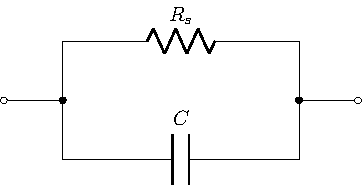
\includegraphics[width=6cm,height=4cm]{Ejercicio_1(Germo)/Circuitos/circuito_equivalente_capacitor.pdf}
\label{fig:circuito_equivalente_capacitor}
\end{figure}
%~circuito equivalente capacitor


La resistencia observada se debe a la resistencia eléctrica del material del componente(film).También, se podría considerar la resistencia propia de los terminales. \par
Por otro lado, se podría considerar una inductancia en el modelo equivalente pero debido al método de fabriacación y por las frecuencias con las que se puede trabajar en el laboratorio no se pudo hallar una frecuencia donde se apreciará un comportamiento de tipo inductivo. El máximo cambio de fase obtenido fue de aproximadamente $4^\circ$ a $13 MHz$.


%% Tabla capacitor
 \begin{center}
 
     \begin{table}[H]
     \centering
     \renewcommand{\arraystretch}{1.1}
     \scalebox{0.8}{
         \begin{tabular}{ c c c c c c c c }
            \hline 
             $\bm{f_P[Hz]}$ &  $\bm{C_P[nF]}$ & $\bm{D}$& $\bm{R_P[S]}$ & $\bm{|Z|[S]}$ & $\bm{\theta}[^\circ]$ \\

             \hline
             10   & 2.2  & 0.000 & 0.00       & 0.14$\mu$   & 89.9  \\
			100  & 2.27 & 0.010 & 0.00       & 1.43$\mu$   & 89.90 \\
			1K   & 2.26 & 0.004 & 0.05$\mu$   & 14.22$\mu$  & 89.80 \\
			5K   & 2.25 & 0.007 & 0.49$\mu$   & 70.73$\mu$  & 89.60 \\
			10K  & 2.24 & 0.007 & 1$\mu$ & 0.14$m$ & 89.56 \\
			20K  & 2.23 & 0.010 & 3$\mu$ & 0.28$m$ & 89.42 \\
			30K  & 2.23 & 0.011 & 5$\mu$  & 0.42$m$    & 89.35 \\
			50K  & 2.22 & 0.013 & 9$\mu$  & 0.70$m$  & 89.28 \\
			75K  & 2.21 & 0.014 & 14$\mu$  & 1.04$m$   & 89.22 \\
			100K & 2.21 & 0.014 & 19$\mu$   & 1.38$m$   & 89.21 \\
			200K & 2.19 & 0.015 & 42$\mu$   & 2.75$m$  & 89.30 \\
			400K & 2.18 & 0.016 & 88$\mu$   & 5.47$m$   & 89.08 \\
			450K & 2.17 & 0.016 & 100$\mu$    & 6.15$m$  & 89.07 \\
			500K & 2.17 & 0.016 & 111$\mu$   & 6.82$m$  & 89.06 \\
			550K & 2.12 & 0.017 & 124$\mu$   & 7.40$m$    & 89.06 \\
			650K & 2.17 & 0.017 & 149$\mu$   & 8.84$m$   & 89.04 \\
			750K & 2.16 & 0.017 & 173$\mu$   & 10.20$m$   & 89.03 \\
			800K & 2.16 & 0.017 & 186$\mu$   & 10.87$m$  & 89.02 \\
			900K & 2.16 & 0.017 & 210$\mu$    & 12.22$m$  & 89.01 \\
			1M   & 2.16 & 0.018 & 240$\mu$    & 13.57$m$  & 89.00 \\
			1M2  & 2.16 & 0.018 & 290$\mu$    & 16.27$m$  & 88.97 \\
			2M   & 2.16 & 0.019 & 520$\mu$    & 27.12$m$ & 88.90 \\
			4M   & 2.2  & 0.023 & 1.270$m$   & 55.38$m$  & 88.68 \\
			7M   & 2.3  & 0.032 & 3.200$m$    & 101.05$m$ & 88.16 \\
			9M   & 2.43 & 0.039 & 0.005   & 0.13  & 87.70 \\
			11M  & 2.63 & 0.050 & 0.009   & 0.18   & 87.10 \\
			12M  & 2.76 & 0.057 & 0.012   & 0.21   & 86.70 \\
			13M  & 2.91 & 0.065 & 0.015   & 0.24   & 86.30 \\
            \hline 
        \end{tabular}
        }
        \caption{Magnitudes del capacitor en función de la frecuencia}
        \label{table:Rta_en_frecuencia_capacitor}
    \end{table}
\end{center}
%%~Tabla capacitor
